\documentclass[10pt,twocolumn,letterpaper]{article}
\usepackage[margin=0.75in,columnsep=0.25in]{geometry}
\usepackage{newtxtext,newtxmath}
\usepackage[T1]{fontenc}
\usepackage{microtype}
\usepackage{graphicx}
\usepackage{booktabs}
\usepackage{multirow}
\usepackage{amsmath}
\usepackage[numbers,sort&compress]{natbib}
\usepackage[font=small,labelfont=bf,skip=4pt]{caption}
\usepackage{xcolor}
\usepackage[colorlinks=true,linkcolor=black,citecolor={blue!50!black},urlcolor={blue!50!black}]{hyperref}
\usepackage{enumitem}
\setlist{nosep,leftmargin=*}
\usepackage{titlesec}
\titlespacing*{\section}{0pt}{6pt}{3pt}
\titlespacing*{\subsection}{0pt}{4pt}{2pt}
\titleformat*{\section}{\large\bfseries}
\titleformat*{\subsection}{\normalsize\bfseries}
\setlength{\emergencystretch}{1.5em}
% generated by scripts/make_figures.py from results/ -- do not edit by hand
\newcommand{\BaseGoal}{20/20 (100\%, CI 84--100)}
\newcommand{\BaseGoalPct}{100\%}
\newcommand{\BaseSpatial}{59/100 (59\%, CI 49--68)}
\newcommand{\BaseSpatialPct}{59\%}
\newcommand{\CamXfifty}{30}
\newcommand{\CamXfiftyCI}{[22, 40]}
\newcommand{\CamXfiftyInterp}{>30}
\newcommand{\CamXfiftyInterpCI}{[15, >30]}
\newcommand{\EvalCheckP}{0.74}
\newcommand{\LangAbsurd}{0/50}
\newcommand{\LangDiag}{25/30 (83\%, CI 66--93)}
\newcommand{\LangEmpty}{0/50}
\newcommand{\LangOffEnv}{0\%}
\newcommand{\LangOffEnvFrac}{0/270}
\newcommand{\LangOffInstructed}{73\%}
\newcommand{\LangOffInstructedFrac}{197/270 (73\%, CI 67--78)}
\newcommand{\LangOther}{2/270}
\newcommand{\LangPara}{35/150 (23\%, CI 17--31)}
\newcommand{\LangParaClose}{20/50}
\newcommand{\LangParaDistant}{4/50}
\newcommand{\LangParaReworded}{11/50}
\newcommand{\LangVariantsFailed}{215}
\newcommand{\LangVariantsFailedAnyGoal}{0}
\newcommand{\LerobotEvalCheck}{14/20 (70\%)}
\newcommand{\LightCliffHigh}{81\%}
\newcommand{\LightCliffLow}{67.5\%}
\newcommand{\LightXfifty}{0.76}
\newcommand{\LightXfiftyCI}{[0.72, 0.81]}
\newcommand{\LightXfiftyInterp}{0.74}
\newcommand{\LightXfiftyInterpCI}{[0.72, 0.78]}
\newcommand{\OurEvalCheck}{12/20 (60\%)}
\newcommand{\RLCleanRes}{8/10}
\newcommand{\RLCleanResPct}{80\%}
\newcommand{\RLCleanVla}{8/10}
\newcommand{\RLCleanVlaPct}{80\%}
\newcommand{\RLSeeds}{1}
\newcommand{\RLStrongRes}{1/10}
\newcommand{\RLStrongResPct}{10\%}
\newcommand{\RLStrongVla}{1/10}
\newcommand{\RLStrongVlaPct}{10\%}
\newcommand{\RLTrainRes}{4/10}
\newcommand{\RLTrainResPct}{40\%}
\newcommand{\RLTrainVla}{5/10}
\newcommand{\RLTrainVlaPct}{50\%}
\newcommand{\RobotXfifty}{0.078}
\newcommand{\RobotXfiftyCI}{[0.05, 0.11]}
\newcommand{\RobotXfiftyInterp}{0.048}
\newcommand{\RobotXfiftyInterpCI}{[0.031, 0.082]}
\newcommand{\TotalEpisodes}{1\,755}

\providecommand{\RLRandConclusion}{A residual corrector trained with a few hundred episodes does not repair the arm-pose weakness on unseen configurations.}

\title{\vspace{-1.2em}\textbf{Does a small VLA listen, and where does it break?}\\[2pt]
\large Graded robustness of SmolVLA on LIBERO and a residual RL correction}
\author{Ana\"is Azouaoui\vspace{-0.6em}}
\date{}

\begin{document}
\maketitle

\begin{abstract}
Vision-language-action (VLA) models are evaluated almost exclusively in the conditions they were
trained on. We probe SmolVLA~\citep{shukor2025smolvla}, a 450M-parameter open VLA, on the LIBERO
benchmark~\citep{liu2023libero} with three questions. \emph{Does it listen?} In LIBERO-Goal, where ten
tasks share one scene, we swap instructions and check all ten goal predicates at every step: the robot
reaches the goal of the instruction it is given in \LangOffInstructed{} of swapped episodes and the
environment's own goal in \LangOffEnv{}, but hand-written paraphrases of the same instruction succeed
far less often (\LangParaPct{} against \LangOrigPct{}). \emph{How does it break?} Under five graded
perturbations, success declines gradually with camera viewpoint, collapses past sharp thresholds for
lighting and pixel noise, and is halved by an offset of about 3$^\circ$ per arm joint at the start of the
episode. \emph{Can a small corrector help?} A residual policy trained with PPO on top of the frozen VLA
improves success on the initial states it was trained on but not on held-out ones, and mostly learns to
finish successful episodes faster. All results come from \TotalEpisodes{} simulated episodes run on a
laptop, with per-episode logs and code released.
\end{abstract}

\section{Introduction}
VLA models map a camera image and a sentence to robot actions with a single network. Benchmark scores
on LIBERO are now close to saturation, which says little about what happens when the scene moves
slightly away from the demonstrations. Recent robustness suites~\citep{fei2025liberoplus,zhou2025liberopro}
answer this with many perturbation types at a few fixed levels and report that models are fragile to
viewpoint and initial state, and largely ignore language.

This report looks at a narrower set of questions in more depth, on one small model:
\begin{itemize}
  \item \textbf{Listening.} If the scene is held fixed and only the instruction changes, does the robot
  change what it does? Checking every task's goal, not only the one the environment scores, separates
  ``ignores the instruction'' from ``follows it but fails''.
  \item \textbf{Shape of the degradation.} Each perturbation has a continuous intensity; we fit a dose-response
  curve and estimate the intensity $x_{50}$ at which success falls to half its unperturbed value.
  \item \textbf{Repair without retraining.} A small policy trained with PPO adds a bounded correction to
  the frozen VLA's actions (residual RL~\citep{silver2018residual,johannink2019residual}).
\end{itemize}

\section{Related work}
\textbf{Robustness of VLAs.} LIBERO-Plus~\citep{fei2025liberoplus} perturbs LIBERO along seven axes
(camera, lighting, language, sensor noise, robot initial state, layout, textures) and finds camera and
initial-state changes the most harmful, and language variations almost harmless, which the authors read
as models ignoring language. LIBERO-PRO~\citep{zhou2025liberopro} reports that success can collapse
under object and position changes and argues that high scores reflect memorisation. We reuse their
perturbation axes but sweep intensity continuously, and our listening test scores every goal of the shared
scene rather than only the environment's own goal.

\textbf{Residual policies.} Residual RL learns a correction on top of a fixed controller or
policy~\citep{silver2018residual,johannink2019residual}; ResiP~\citep{ankile2024resip} and Policy
Decorator~\citep{yuan2024policydecorator} apply it to imitation-learned diffusion or transformer policies.
We apply the same idea to a VLA, targeting one specific robustness failure.

\section{Setup}
\textbf{Model and simulator.} We use the Hub checkpoint \texttt{lerobot/smolvla\_libero} (revision
\texttt{31d453f}), evaluated through LeRobot~\citep{cadene2024lerobot} 0.6.1 processors so that
normalisation, tokenisation and camera naming match \texttt{lerobot-eval}. The policy predicts chunks of
50 relative end-effector actions with flow matching~\citep{lipmanflow2022} and executes the whole chunk
before re-planning. Images are $360\times360$ from the third-person (\emph{agentview}) and wrist cameras.
Everything ran on an Apple M1 laptop (8\,GB, PyTorch MPS, bf16 weights); LIBERO runs natively on macOS once
an unused Linux-only dependency is skipped.

\textbf{Protocol.} Episode $e$ of a task always starts from LIBERO initial state $e$ with seed $e$ (which
also fixes the flow-matching noise), whatever the condition, so conditions are compared on identical
episodes. Hard resets are used throughout. Success rates are reported with Wilson 95\% intervals~\citep{wilson1927};
paired comparisons use an exact McNemar test.

\begin{figure}[t]
  \centering
  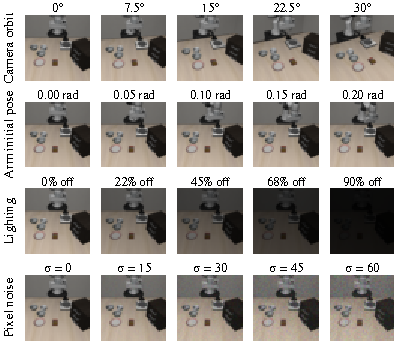
\includegraphics[width=\columnwidth]{figures/perturbation_grid.pdf}
  \caption{What the policy sees from the main camera at intensities 0, 0.25, 0.5, 0.75 and 1
  (LIBERO-Spatial task 0, initial state 0). The arm offset also moves the wrist view (not shown).}
  \label{fig:grid}
\end{figure}

\textbf{Perturbations} (Fig.~\ref{fig:grid}). \emph{Camera orbit}: the agentview camera rotates about the
vertical axis through the point it looks at on the table, $0$--$60^\circ$, sign alternating with the
episode; the wrist camera is untouched. \emph{Arm initial pose}: after reset, each of the seven joints
is shifted by $\pm\delta$, $\delta\in[0,0.2]$\,rad, with signs drawn per episode; objects are not moved.
\emph{Lighting}: every light in the scene is scaled down by up to 90\%. \emph{Pixel noise}: Gaussian noise
of standard deviation up to 60 grey levels on both cameras. At the strongest level all task-relevant
objects remain visible (Fig.~\ref{fig:grid}), except at 90\% light removal where the scene is very dark
but still readable.

\textbf{Dose-response fit.} For each perturbation we fit
$p(x) = s_0 / (1 + e^{(x - x_{50})/w})$ by binomial maximum likelihood, with $s_0$ fixed to the
unperturbed success rate on the same episodes, so that $x_{50}$ is exactly the intensity at which
success is halved. Its 95\% interval comes from a bootstrap over tasks (whole tasks resampled), since
task difficulty varies far more than episode outcomes within a task.

\section{Results}

\textbf{Baseline.} Without perturbation SmolVLA succeeds in \BaseSpatial{} LIBERO-Spatial episodes
(10 tasks $\times$ 10) and in \BaseGoal{} LIBERO-Goal episodes. The Spatial rate is well below the 90\%
reported in~\citep{shukor2025smolvla}. To rule out our own evaluation loop, we re-ran two tasks with the
official \texttt{lerobot-eval}: \LerobotEvalCheck{}, against \OurEvalCheck{} with our loop on the same
tasks, a difference well within sampling noise. Two tasks (5 and 8) are solved in at most 2 of 10
episodes. All conclusions below are relative to this measured baseline.

\begin{figure*}[t]
  \centering
  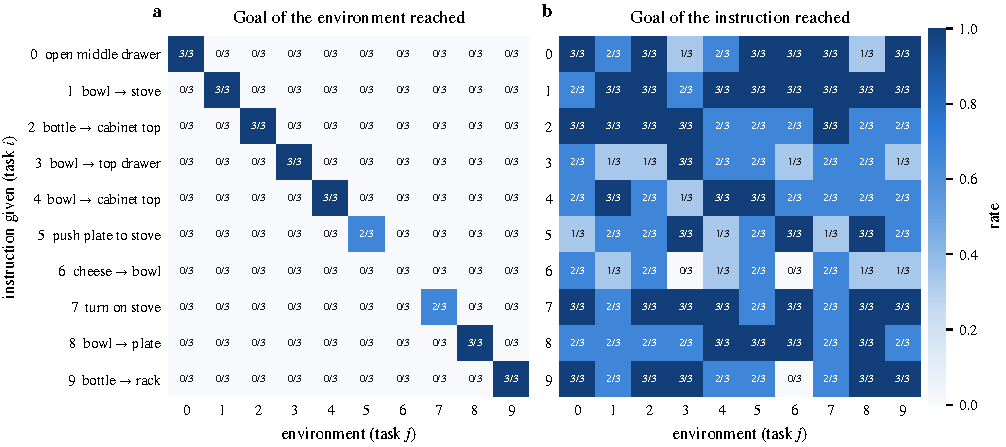
\includegraphics[width=\textwidth]{figures/language_matrix.pdf}
  \caption{\textbf{Listening test on LIBERO-Goal} (3 episodes per cell). The environment of task $j$ is
  built and the instruction of task $i$ is given. (a)~Success as scored by the environment (goal $j$).
  (b)~Whether the goal of the \emph{given} instruction $i$ was reached at any point of the episode,
  obtained by evaluating all ten goal predicates of the shared scene at every step. Off the diagonal
  the robot never completes the environment's own task, but reaches the instructed goal in
  \LangOffInstructedFrac{} of episodes.}
  \label{fig:language}
\end{figure*}

\subsection{SmolVLA follows the instruction}
Fig.~\ref{fig:language}a is the matrix one would get from the environment alone: success only on the
diagonal. Read in isolation it is ambiguous, since a robot that ignores language would also fail
off-diagonal if it performed some fixed behaviour unrelated to goal $j$. Panel~(b) removes the
ambiguity. When told to do task $i$ inside the environment of task $j$, the robot reaches goal $i$
in \LangOffInstructed{} of the 270 swapped episodes, close to the \LangDiag{} obtained with matched
instructions, and reaches the environment's goal in \LangOffEnvFrac{} of them; only \LangOther{}
episodes complete a third, unrelated goal. The initial states of the ten tasks differ slightly (each task
has its own set), so the robot is not keyed on the start configuration either. The weakest instructions
are those whose objects are close to other objects (task 3, bowl into the top drawer; task 6, cream
cheese into the bowl).

This contrasts with the conclusion of LIBERO-Plus that VLAs largely ignore language. A swap test
is a direct check: in a fixed scene, only the instruction can tell the robot which of ten goals to
pursue.

\begin{figure}[t]
  \centering
  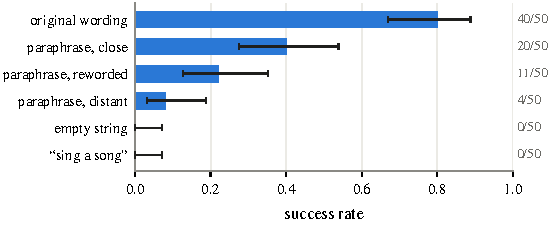
\includegraphics[width=\columnwidth]{figures/language_variants.pdf}
  \caption{\textbf{Instruction variants} on LIBERO-Goal (environment and instruction of the same
  task, 5 episodes per task). Paraphrases were written by hand, from close to the original wording
  to fully reworded. Wilson 95\% intervals.}
  \label{fig:variants}
\end{figure}

\subsection{\dots{} but to the exact words}
The same model is brittle to rewording (Fig.~\ref{fig:variants}). Hand-written paraphrases that keep
the goal unchanged succeed in only \LangPara{} of episodes, against \LangOrig{} with the original
wording on the same episodes, and the rate drops with the distance from
the training wording: \LangParaClose{} for a close paraphrase (\emph{``place the bowl on the
stove''}), \LangParaReworded{} for a reworded one, \LangParaDistant{} for the most distant. Small
changes matter: \emph{``turn the stove on''} works, \emph{``switch on the stove''} does not. An empty
instruction and an unrelated one (\emph{``sing a song''}) both give \LangEmpty{}. In none of the
\LangVariantsFailed{} failed episodes does the robot complete any of the ten goals: without an
instruction it recognises, it does not fall back on a default task, it does nothing useful.

Taken together, the instruction is what selects the behaviour, but it acts more like a key into a
small set of learned behaviours than like language that is understood. For this model and suite we
therefore find sensitivity to language on both counts: naming another goal changes the behaviour, and
rewording the same goal breaks it. Model, suite and perturbation types all differ from LIBERO-Plus,
and we did not reproduce their setting, so this is a statement about SmolVLA on LIBERO-Goal only.

\textbf{A fix at the input.} Mapping each instruction to the closest of the 40 LIBERO training
instructions with a sentence encoder (all-MiniLM-L6-v2~\citep{reimers2019sbert}; below a cosine
similarity of \CanonThreshold{}, fixed beforehand, the instruction is left unchanged) brings paraphrases from
\CanonGoalRaw{} to \CanonGoal{} on LIBERO-Goal, the level of the original wording, and rejects
\emph{``sing a song''}. On LIBERO-Spatial, where instructions differ only by a spatial relation, the
encoder confuses \textit{next to} and \textit{on} for 5 of 20 paraphrases and success only rises from
\CanonSpatialRaw{} to \CanonSpatial{}.

\begin{figure*}[t]
  \centering
  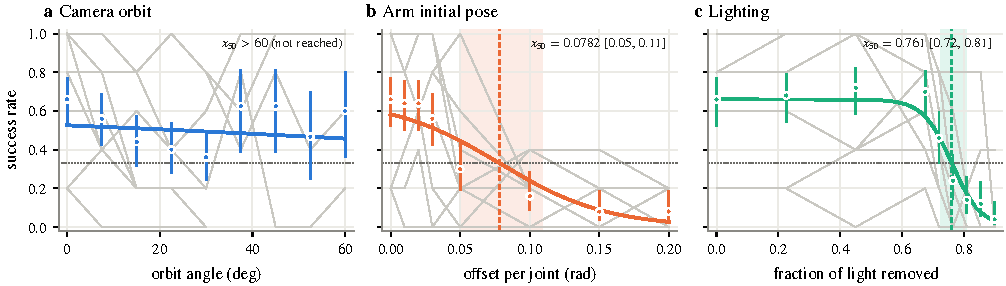
\includegraphics[width=\textwidth]{figures/dose_response.pdf}
  \caption{\textbf{Success versus perturbation intensity} on LIBERO-Spatial (10 tasks, 5 episodes per
  task and level; the unperturbed point uses the same episodes). Dots: pooled success with Wilson 95\%
  intervals. Grey: individual tasks. Line: logistic fit with $s_0$ fixed to the unperturbed rate; dotted:
  half of it. Dashed line and band: breaking point $x_{50}$ and its 95\% task-bootstrap interval.}
  \label{fig:dose}
\end{figure*}

\subsection{Different ways of breaking}
The perturbations do not just differ in strength; the curves have different shapes (Fig.~\ref{fig:dose}).
We report two estimates of the breaking point: the logistic $x_{50}$, and a model-free one (pooled
success made non-increasing by isotonic regression, then linearly interpolated at half the baseline),
both with task-bootstrap intervals.
\begin{itemize}
  \item \textbf{Camera orbit: gradual.} Success declines steadily with the angle, with no plateau and no
  cliff: it is halved around $x_{50}=\CamXfifty^\circ$ \CamXfiftyCI{} and is still above zero at
  $60^\circ$, a viewpoint far from anything in the demonstrations. The decline is strongly task
  dependent: some tasks are unaffected at the largest angle, others fail from the first level. The two
  orbit directions are not equally harmful at intermediate angles, but direction is confounded with the
  initial state here (it alternates with the episode index), so we do not interpret it.
  \item \textbf{Arm initial pose: narrow tolerance, then a cliff.} Offsets up to 0.02\,rad per joint
  ($\approx1^\circ$) leave success unchanged; between 0.03 and 0.05\,rad it is halved (model-free
  $x_{50}=\RobotXfiftyInterp$\,rad \RobotXfiftyInterpCI{}; logistic \RobotXfifty{}\,rad), and a long tail
  follows. The objects have not moved and the wrist camera still sees them; the policy only starts
  from an arm configuration a few degrees away from the demonstrations.
  \item \textbf{Lighting: threshold.} Removing up to \LightCliffLow{} of the light has no measurable
  effect; success is then halved at $x_{50}=\LightXfiftyInterp$ \LightXfiftyInterpCI{} of light removed
  and falls below a quarter of the baseline at \LightCliffHigh{}. A single fixed-level test would either
  miss the effect entirely or report a collapse.
  \item \textbf{Pixel noise: threshold.} No effect at a standard deviation of 15 grey levels, a small
  one at 30, then a collapse: success is halved at $x_{50}=\NoiseXfiftyInterp$ \NoiseXfiftyInterpCI{} and is
  close to zero at 60, although the objects remain easy to see for a human at that level
  (Fig.~\ref{fig:grid}).
\end{itemize}
Gradual decline for viewpoint, sharp thresholds for photometric changes (lighting, noise) and a narrow
tolerance for the arm configuration: one fixed perturbation level per axis would have placed these on a
single ``robust/fragile'' scale and missed the differences.
\textbf{Both cameras are needed.} Blacking out one stream entirely drops success from \CamMaskBoth{} to
\CamMaskAgent{} without the main camera and \CamMaskWrist{} without the wrist camera (same episodes). The
policy cannot do without the third-person view, yet tolerates rotating it by $20$--$30^\circ$ with a
moderate loss, which suggests it relies on coarse scene layout from that view rather than on precise
image coordinates.

\textbf{Harmless alone, harmful together.} We restrict each perturbation to a range where it alone costs at
most about 15\% of the baseline (camera $\le7.5^\circ$, arm $\le0.03$\,rad, light removed $\le67.5\%$,
noise $\sigma\le30$) and keep the 15 episodes that succeed under each one alone at the top of its range. A
MAP-Elites search~\citep{mouret2015mapelites} over their combinations (\QDEvals{} combinations, four search
episodes each) finds failures almost everywhere: \QDAnyFail{} combinations fail at least one episode, the
full combination fails \QDCornerFails{}, and the six most harmful ones make \QDValPooled{} of the 11 held-out
episodes fail. One-factor-at-a-time curves overestimate the margin when several conditions drift together.

\begin{figure*}[t]
  \centering
  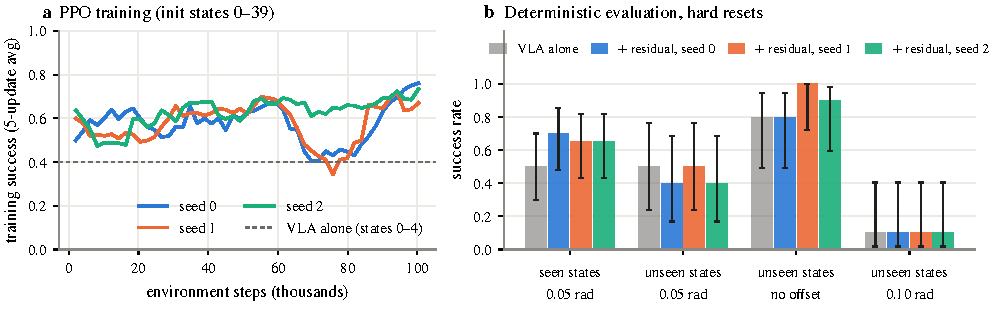
\includegraphics[width=\textwidth]{figures/rl_residual.pdf}
  \caption{\textbf{Residual RL on the arm-offset weakness} (LIBERO-Spatial task 2, offset 0.05\,rad per
  joint). (a)~Success of the stochastic policy during PPO, moving average over 5 updates (about 60
  episodes). (b)~Deterministic evaluation with hard resets, on initial states seen during training
  (0--19, 20 episodes) and on held-out ones (40--49, 10 episodes per bar). Wilson 95\% intervals.}
  \label{fig:rl}
\end{figure*}

\subsection{A residual corrector learns, but does not generalise}
\textbf{Target and design.} The arm-offset weakness is a natural target: the perturbation is visible in
proprioception, so a corrector without images can in principle detect it. We use LIBERO-Spatial task 2
at 0.05\,rad per joint, where the VLA alone succeeds in about half of the episodes. The corrector is an MLP
(two hidden layers of 128) that sees end-effector position and orientation, gripper opening, the VLA's
proposed action and the episode progress, and outputs $\Delta a\in[-1,1]^7$; the executed action is
$\mathrm{clip}(a_{\mathrm{VLA}} + 0.2\,\Delta a)$. Its last layer is initialised to zero, so before
training it reproduces the VLA exactly; we checked this on full episodes (identical outcomes and episode
lengths). It is trained with PPO~\citep{schulman2017ppo} in a single-file implementation in the style of
CleanRL~\citep{huang2022cleanrl}, with a sparse reward (1 on success), $\gamma=0.995$, four simulators in
one process sharing batched VLA calls, and 100k environment steps per run (about 400 episodes, 3\,h on
the laptop at 10 steps/s). Training uses initial states 0--39; states 40--49 are kept for evaluation.

\textbf{Results} (Fig.~\ref{fig:rl}). Training success rises modestly (from \RLTrainFirst{} to
\RLTrainLast{} over the first and last ten updates of each of the \RLSeeds{} seeds); seeds 0 and 1 dip around 70k steps before recovering, seed 2 does not. On initial states seen in training, the deterministic corrector succeeds in
\RLSeenRes{} episodes against \RLSeenVla{} for the VLA alone, and every discordant episode favours the
corrector (McNemar $p=$ \RLPSeen{}, not significant at this sample size). On held-out initial states the
gain disappears: \RLUnseenRes{} against \RLUnseenVla{} at the training level, \RLUnseenStrongRes{} against
\RLUnseenStrongVla{} at 0.10\,rad, and \RLUnseenCleanRes{} against \RLUnseenCleanVla{} without offset
(so the corrector does not hurt the unperturbed task).

What does transfer is speed: successful episodes are shorter with the corrector, from \RLStepsSeenVla{} to
\RLStepsSeenRes{} steps on seen states and from \RLStepsUnseenVla{} to \RLStepsUnseenRes{} on held-out
ones. This is what the objective rewards most directly: with discounting a faster success is worth more,
and speeding up an episode that already works is observed in every rollout, whereas recovering a failure
is a rare event in 400 episodes. The recoveries that do happen are tied to the configurations seen in
training; with 40 of them, the corrector has little to interpolate from.

Drawing new offset signs at every training reset, to expose the corrector to more varied starting poses,
gives the same pattern (\RLRandSeenRes{} on seen and \RLRandUnseenRes{} on held-out initial states), so the
variety of arm offsets is not what limits generalisation.

A training-free alternative, executing 10 instead of 50 actions per chunk so that the VLA re-plans five
times more often, gives \RLReplanClean{}, \RLReplanTrain{} and \RLReplanStrong{} on the same held-out
episodes (no offset, 0.05 and 0.10\,rad), not distinguishable from the VLA alone with 10 episodes, at
\RLReplanSlowdown{}$\times$ the cost.



\section{Limitations}
Everything is in simulation, on one model and one checkpoint, with 3--10 episodes per cell; intervals are
correspondingly wide and per-task curves noisy. Our baseline is well below the numbers reported in the
SmolVLA paper (which may not use this Hub checkpoint), so all conclusions are relative to the measured
baseline. Inference ran on Apple MPS in bf16; a GPU run with the same configs is provided but was not used
for the reported numbers. The residual corrector sees proprioception only, which is why we target a
perturbation that is visible in proprioception.

\section{Conclusion}
On LIBERO, SmolVLA is neither deaf to language nor robust to it: the instruction decides which task is
attempted, but only in wordings close to the training ones. Its failures under distribution shift have
distinct shapes, gradual for viewpoint and abrupt for photometric changes and arm configuration,
which a single perturbation level per axis would hide. A residual corrector trained with a few hundred
episodes does not repair the arm-pose weakness on unseen configurations; making it generalise likely
requires many more initial states, or an input that encodes the scene rather than proprioception only.
Natural next steps are a search over combinations of perturbations rather than one axis at a time, and
the same protocol on larger VLAs.


{\small
\bibliographystyle{abbrvnat}
\setlength{\bibsep}{1pt}
\bibliography{refs}
}
\end{document}
